\documentclass{beamer}
\usepackage[english,russian]{babel}
\usepackage[utf8]{inputenc}
\usepackage{amsmath}
\usepackage{hyperref}
\usetheme{Warsaw}
\usepackage{listings}
\usepackage{xcolor}
\usepackage{tikz}
\usetikzlibrary{graphs}
\usepackage{algpseudocode}

\lstset{
    frame=tb,
    tabsize=4,
    showstringspaces=false,
    numbers=left,
    commentstyle=\color{green},
    keywordstyle=\color{blue},
    stringstyle=\color{red},
    emph={baz},
    emphstyle=\textbf
}
\begin{document}

\title{SAT/SMT solvers\ \newline 13. Bounded Model Checking}
\author{Roman Kholin}
\institute{Lomonosov Moscow State University}
\date{Moscow, 2023}

\begin{frame}
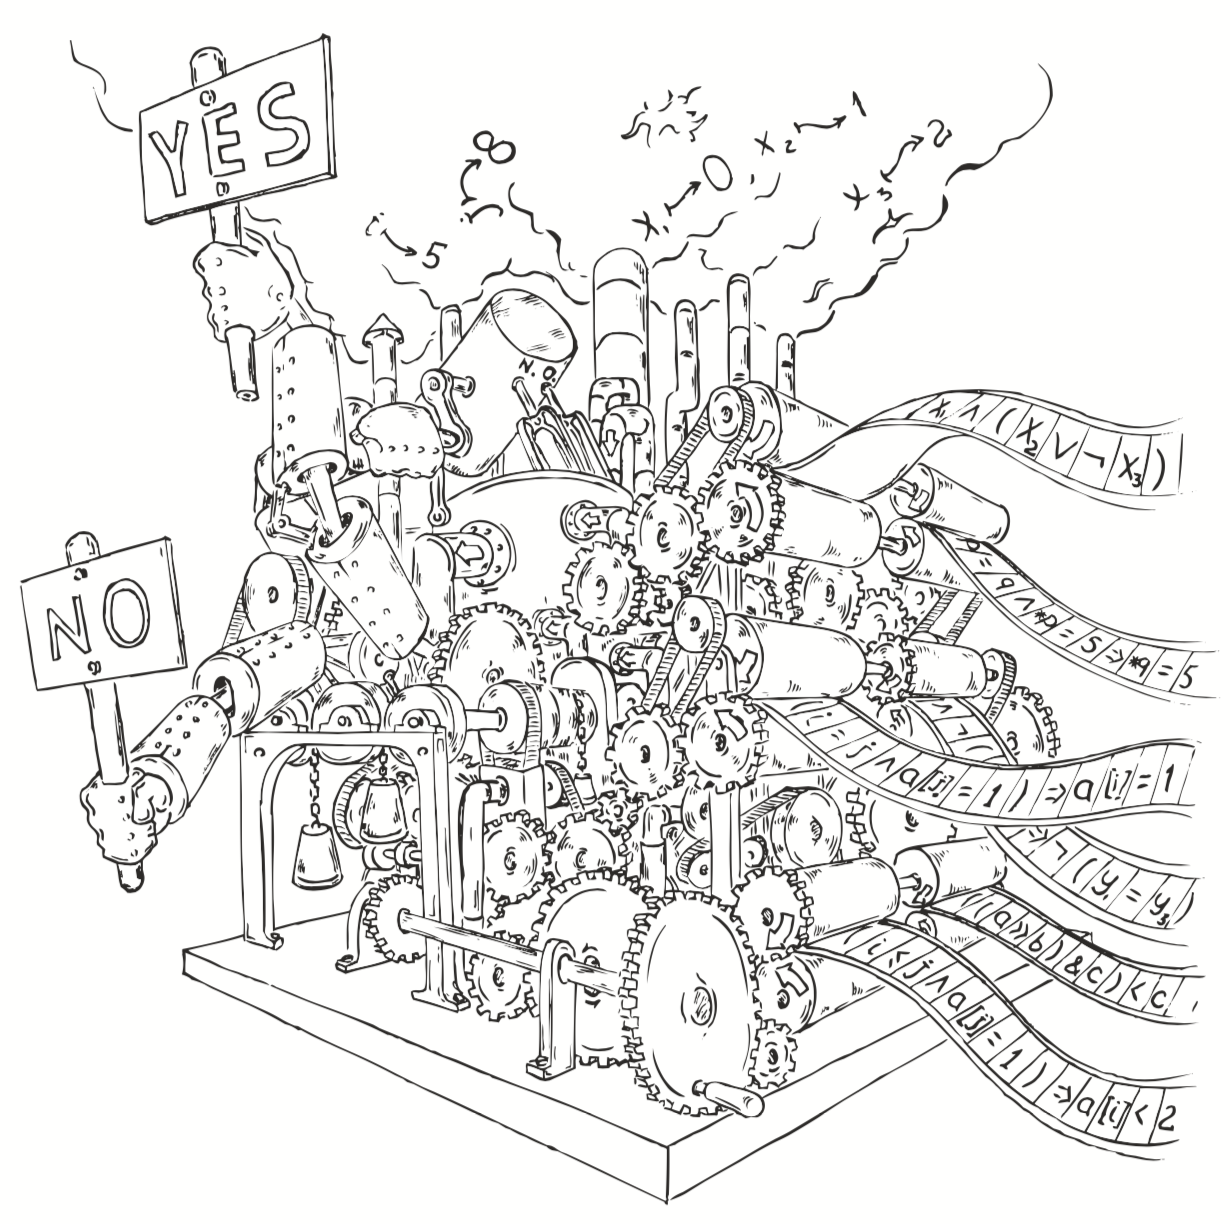
\includegraphics[scale=0.5]{../decision-procedure.png}
\end{frame}

\frame{\titlepage}

\begin{frame}{Kripke Structures}
\begin{itemize}
\item $K = (S, S_0, L, T)$
\item $S$ is a (finite) set of states
\item $S_0$ is a start state
\item $L: S \rightarrow 2^V$ is a labelling function that maps each state to the set of propositional variables that hold in it
\item $T \subseteq S\times S$ is a total transition relation
\end{itemize}
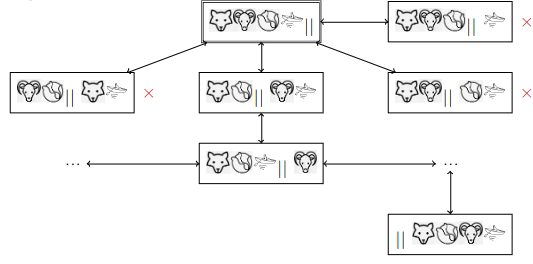
\includegraphics[scale=0.5]{wolf.png}
\end{frame}

\begin{frame}{Big number of states}
2 Variables\newline
2 Buffers\newline
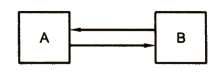
\includegraphics[scale=0.5]{ex1.png}
\end{frame}

\begin{frame}{Symbolic Model Checking}
\begin{itemize}
\item $M = (S, S_0, L, T)$
\item $S = \{s_0, s_1, s_2\}$
\item $S_0 = \{s_0\}$
\item $T = \{(s_0, s_1), (s_0, s_2), (s_1, s_0), (s_1, s_2), (s_2, s_2)\}$
\item predicats: $\{p, q, r\}$
\item $Sat_p = \{s_0\}, Sat_q = \{s_0, s_1\}, Sat_r = \{s_1, s_2\}$
\end{itemize}
\end{frame}

\begin{frame}{Symbolic Model Checking}
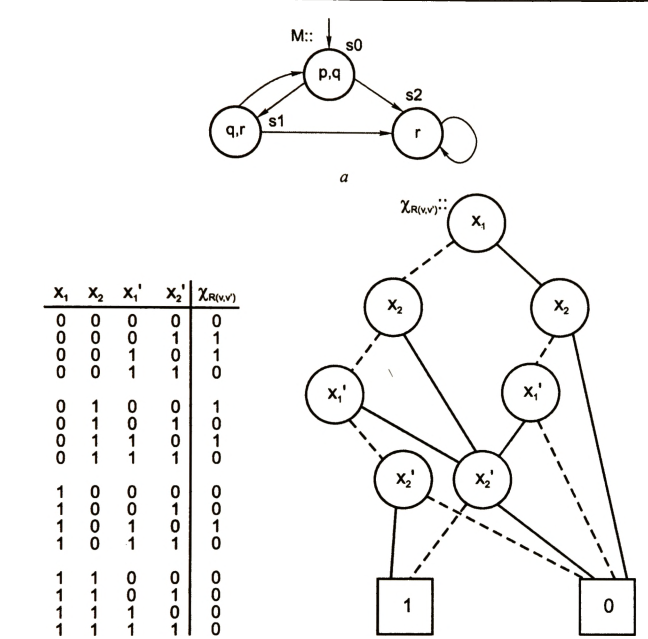
\includegraphics[scale=0.35]{smb_ex.png}
\end{frame}

\begin{frame}{Symbolic Model Checking}
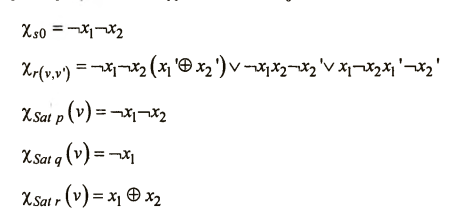
\includegraphics[scale=0.5]{smb_ex_formula.png}
\end{frame}

\begin{frame}{Symbolic Model Checking}
\begin{itemize}
\item Initial state: $S_0: \lnot l \wedge \lnot r$
\item Transition: $T: (l' = (l\neq r)) \wedge (r' = \lnot r)$
\item Property:$ \lnot l \vee \lnot r$
\end{itemize}
\end{frame}

\begin{frame}{Linear Temporal Logic}
Path: $\pi = (s_0, s_1, \dots )$\newline
Suffix: $\pi^i = (s_i, s_1, \dots )$\newline
Temporal operators are the: <<next time>> operator \textbf{X}, the <<finally>> operator \textbf{F}, the <<globally>> operator \textbf{G}\newline
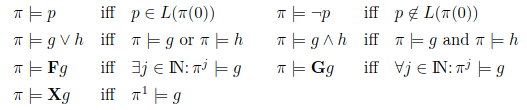
\includegraphics[scale=0.5]{ltl.png}\newline
$\lnot \textbf{F}g = $\newline
$\lnot \textbf{G}g = $\newline
$\lnot \textbf{X}g = $
\end{frame}

\begin{frame}{Temporal properties}
\begin{itemize}
\item "Safety" properties
    \begin{itemize}
    \item "Always x=y"\newline
          $(\textbf{G}(x=y))$
    \item "Every Send is followed by Ack"\newline
          $(\textbf{G}(Send \rightarrow \textbf{F} Ack))$
    \end{itemize}
\item "Liveness" properties
    \begin{itemize}
    \item "Reset can always be reached"\newline
          $(\textbf{GF}Reset)$
    \item "From some point on, always switch\_on"\newline
          $(\textbf{FG} switch\_on)$
    \end{itemize}
\end{itemize}
\end{frame}

\begin{frame}{Bounded Model Checking}
\begin{itemize}
\item Based on SAT
\item $\exists$ Counterexample of length $k \iff$ Propositional Formula is satisifiable
\item BMC for LTL reduced to SAT in poly time
\item Advantages:
\begin{itemize}
\item CounterExamples – found fast, minimal length
\item Less space, No manual ordering ( vs BDD )
\item The best SAT solvers are capable of handling thousands of state variables
\end{itemize}
\item Disadvantages
\begin{itemize}
\item with the limit k, completeness is naturally sacrificed
\end{itemize}
\end{itemize}
\end{frame}

\begin{frame}{Bounded Semantics}
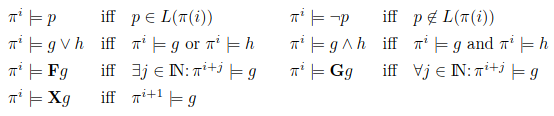
\includegraphics[scale=0.5]{bs1.png}
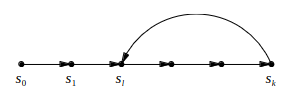
\includegraphics[scale=0.5]{lasso.png}
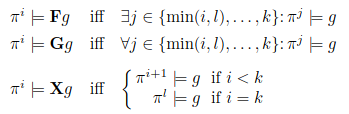
\includegraphics[scale=0.5]{bs2.png}
\end{frame}

\begin{frame}{Example}
Most safety properties can be reduced to "Always $p$" where $p$ is propositional\newline
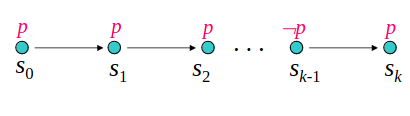
\includegraphics[scale=0.5]{ex2.png}
\end{frame}

\begin{frame}{SAT}
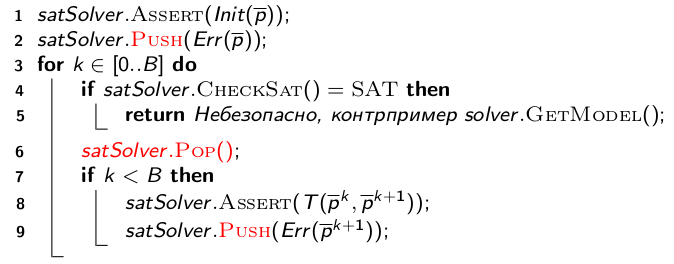
\includegraphics[scale=0.5]{sat.png}
\end{frame}

\begin{frame}{Encoding}
With loop:\newline
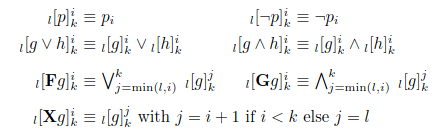
\includegraphics[scale=0.5]{not_loop.png}\newline
Without loop:\newline
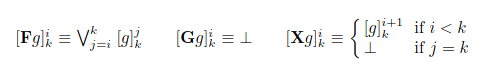
\includegraphics[scale=0.5]{loop.png}\newline
Result:\newline

\includegraphics[scale=0.5]{result.png}
\end{frame}

\begin{frame}{Determining the Bound}
\begin{itemize}
\item Theorem: for \textbf{G}p properties Completeness Threshold is Diameter - longest "shortest path" from an initial state to any other reachable state
\item Theorem: for \textbf{F}p properties Completeness Threshold is Recurrence Diameter - longest loop-free path
\item Open Problem: The value of Completeness Threshold for general Linear Temporal Logic properties is unknown
\end{itemize}
\end{frame}

\begin{frame}
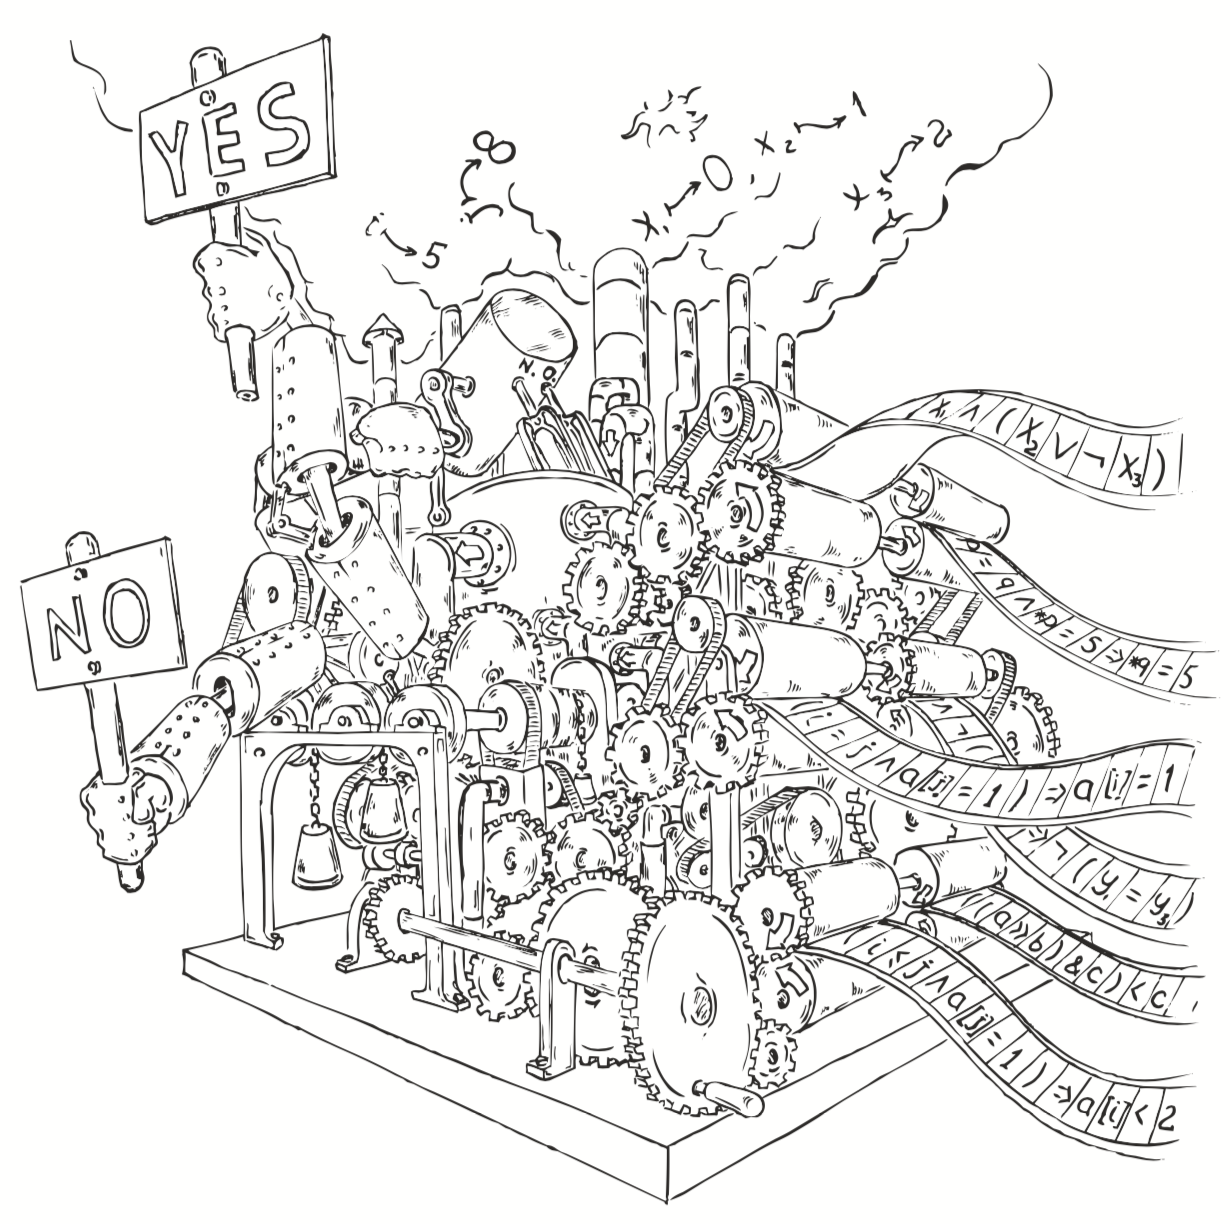
\includegraphics[scale=0.5]{../decision-procedure.png}
\end{frame}

\end{document}
